%% ----------------------------------------------------------------
%% Background.tex
%% ---------------------------------------------------------------- 
\chapter{Theoretical Background} \label{Chapter:Background}

\section{Machine Learning}

Machine learning focuses on developing algorithms and models that enable computers to learn patterns from data and make predictions or decisions without being explicitly programmed for the task \cite{Murphy}. 
The use of statistical techniques such as linear regression allows it to improve its performance over time as it is exposed to more information. 
There are three commonly used machine learning approaches \cite{Bishop} including supervised learning, where the algorithm is trained on labeled data; 
unsupervised learning, where the algorithm discovers patterns in unlabeled data; and reinforcement learning, where the algorithms learn through trial and error based on feedback from its actions.

\subsection{Performance Measure}

To let computers learn the patterns from data, minimising the cost function is often the target. This function measures how close the predictions are made to the actual targets, and gives an idea of how well the performance is. 
In this project, mean squared error (MSE) and mean absolute percentage error (MAPE) have been considered as cost functions. The functions of the two indicators are shown below:
\begin{gather}
    \mathrm{MSE} = \frac{1}{n}\sum_{i=1}^{n}(\hat{y_i} -y_i)^2 
\end{gather}
The MSE calculates the square of the difference between the predicted value $\hat{y_i}$ and the actual value $y_i$, and takes the mean of it \cite{Bishop}. 
The value is in the range of $[0, +\infty)$, when the predicted value equals the real value, MSE is 0. As the difference gets larger, MSE increases. 
\begin{gather}
    \mathrm{MAPE} = \frac{100\%}{n} \sum_{i=1}^{n} \left | \frac{\hat{y_i}-y_i}{y_i} \right | 
\end{gather}
Instead of the actual value of the loss, MAPE is focused on the relative difference \cite{Hyndman}. The range of MAPE is also $[0, +\infty)$, where a 0\% MAPE means a perfect match, and above 100\% would be considered as bad. 
In general, if the MAPE is between 5\% and 10\%, it can be considered a good prediction accuracy.
Note that when the real value is in the denominator, which means it is not usable for any data set that contains a real value of 0.

\subsection{Gradient Descent}

Gradient descent is a widely used optimisation algorithm used to minimise the cost function iteratively. It is also a key methodology in both machine learning and deep learning. 
The gradient or derivative of the cost function at a point tells the direction of the steepest increase of the function. 
Hence if the parameters repeatedly update in the opposite direction of the gradient, the model will be closer to, and potentially reach the minimum cost. 
The size of a step of each update is specified by the learning rate. 

For example in linear regression, we shell fit the data using a polynomial function \cite{Bishop}: 
\begin{gather}
    \hat{y}(x, \mathbf{w}) = \omega _0 + \omega _1x^1 + \omega _2x^2 + \dots +\omega _nx^n = \sum_{i=0}^{n}\omega _ix^i 
\end{gather}
where the function has an order of $n$, with $n+1$ parameters $\omega_i$ indicating the significance of each term. These parameters are also denoted as vector $\mathbf{w}$ for future convenience.
The cost function using MSE hence can be denoted as:
\begin{gather}
    \mathrm{MSE} = \frac{1}{n}\sum_{i=1}^{n}(\hat{y}(x_i, \mathbf{w}) - y_i)^2 
\end{gather}
A step of gradient descent can be represented as below, where $\eta$ is the learning rate. 
Repeat the process until it achieves a certain level of accuracy, or other convergence criteria, the polynomial will finally fit the data.
\begin{gather}
    \omega_{new} = \omega_{old} - \eta  \cdot \nabla \mathrm{MSE}
\end{gather}

During gradient descent, local minimum points are often encountered. A local minimum point refers to a point in the cost function which is smaller than its adjacent points, but not the minimum point of the entire cost function.
When using gradient descent for optimisation, the algorithm may converge to such a local minimum. This situation usually occurs when the function has multiple local minima points, and the gradient descent algorithm may be limited by the choice of initial values and the direction of the local gradient. 
In order to solve this problem, some strategies can be adopted, such as running the algorithm multiple times and selecting the smallest result as the final result, or using improved gradient descent algorithms, such as stochastic gradient descent (SGD), momentum method (Momentum), Adam, etc.

\subsection{Overfitting \& Underfitting}

Overfitting and underfitting are common problems in machine learning. They both refer to the situation where the model fails to generalise well to unseen data during training. 

Overfitting stands for the situation when the performance of training data is better than the unseen data. In this case, the model learns noise and subtle patterns in training data, so that it cannot perform the same with another dataset. 
Such a model is overly sensitive to specific examples in the training set. Underfitting, on the other hand, refers to the situation when the model performs poorly on both training data and unseen data. 
The model does not capture patterns and relationships in the data well. This may be because the model is too simple for such a problem. 
Underfit models cannot adapt well to the complexity of the data. 

Overfitting could be eased by regularisation \cite{Santos_2022}, which adds a penalty term to the cost function; increasing the diversity of the training data and reducing the dependence on specific data; and early stopping which monitors the performance of the model and stops training when the performance on unseen data no longer improve. 
The solution to underfitting is rather simple. It could increase the model's complexity, add more features, and increase the amount of training data.

\section{Deep Learning}

Deep learning is a subset of machine learning, focused on large and complex datasets. 
Deep learning is the process of learning the inherent patterns of data, extracting information from text, images, sounds and so on. 
The goal is to enable machines to have a similar analytical learning capabilities as humans. 
Popular deep learning architectures include convolutional neural networks (CNNs), recurrent neural networks (RNNs), and transformers.

Deep learning methods are used in this project due to it enables the computer to learn the patterns from historical traffic data, and make predictions based on those patterns.

\subsection{Neural Network}

At the core of deep learning are artificial neural networks (ANN), which are inspired by the structure and functioning of the human brain. 
The structure of a neural network is illustrated in \fref{Figure:ANN-structure}. It is composed of layers of interconnected nodes (neurons). 
The input layer is where the data is fed into the network, and the output layer produces the final result. Between the input and output layers, there are one or more hidden layers 
each node in the hidden layers has a usually non-linear activation function $A_k$. Section \ref{Section:activation} explains them more. Lines between layers represent linear transformations, 
with the parameter vectors $\mathbf{w}$, and bias $\mathrm{b}$. 

\begin{figure}[!htb]
    \centering
    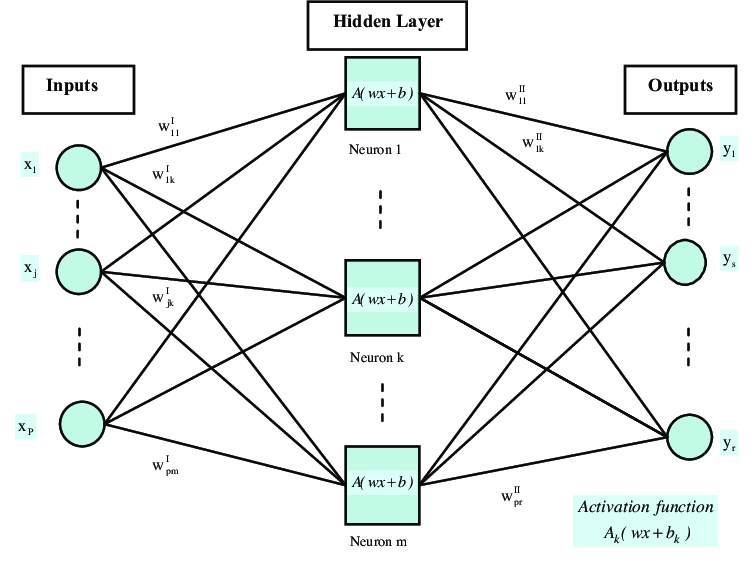
\includegraphics[width=12cm]{ANN-structure}
    \caption{A simple ANN structure with one hidden layer (Adapted from \cite{Koc})}
    \label{Figure:ANN-structure}
\end{figure}

What the network is trying to do is the same as machine learning: find a function that best fits the data, so it can make predictions. The process could be expressed as:
\begin{gather}
    \mathbf{h} = A_k(\mathbf{w^Ix} + b^I_k),\quad k = 1, 2, ..., m \label{eq:single-layer}
\\ \mathbf{y} =\mathbf{w^{II}} \cdot \mathbf{h} + b^{II} \notag
\end{gather}
The inputs fed into the network first go through a linear transformation and then map to an activation function. At last, go through a linear transformation again and output. 
By altering the parameters and the number of hidden layers, it is possible to construct any curve. 

Deep learning emphasises the use of deep neural networks, which means networks with multiple hidden layers. \
These networks are capable of learning complex datasets with non-intuitive characteristics. 
Equation \ref{eq:single-layer} describing a single layer is constant along certain parallel hyperplanes \cite{Pinkus_1999}, hence cannot be used to approximate high-order discontinuous complex functions.
Whereas a two-layer network theoretically can form any complex functions. 
For a particular activation function, it's possible to construct a two-hidden-layer neural network that can approximate any continuous function defined on the unit cube in $\mathbb{R}^n$ to arbitrary precision. 
Specifically, this neural network would have $2n+1$ units in the first hidden layer and $4n+3$ units in the second hidden layer.
Here $n$ is the dimension. The proof could be found in \cite{HECHTNIELSEN199265}.

The model with more than two hidden layers are not unnecessary. 
A deep network can reduce the need for the numbers of nodes in each layer \cite{Poggio2016WhyAW}. 

\subsection{Activation Functions} \label{Section:activation}

The choice of activation function is vital in neural networks. 
It introduces non-linearity into the model \cite{activation}, and enables the network to learn complex patterns and relationships in the data. 
Not all non-linear functions are suitable as activation functions. The process of gradient descent requires the activation function to be differentiable so that the gradients can be calculated. 
Furthermore, in order to better train the neural network, the activation function is preferably monotonically increasing or monotonically decreasing, which can ensure the stability of the gradient.
ReLU is a frequently used example that meets those requirements. 

\subsubsection{Rectified Linear Unit (ReLU)}

ReLU is one of the most commonly used activation functions. It replaces all negative values in the inputs with zero, which can be represented by: 
\begin{gather}
    A(x) = \mathrm{max}(0, x) 
\end{gather}
During the training, it will not activate all neurons at the same time, which gives an advantage that it is computationally efficient.
However, when $x < 0$, the gradient is zero. As training progresses, neurons may become inactive and weights fail to update.
To address this issue, a variant of ReLU, Leaky ReLU, could be used instead. Leaky ReLU allows a small, non-zero gradient when the input is negative.
\begin{gather}
    A(x) = \mathrm{max}(\alpha x, x) 
\end{gather}
where $\alpha$ is a small positive constant. A plot of both functions is shown in \fref{Figure:ReLUplots}

\begin{figure}[!htb]
    \centering
    \subcaptionbox{ReLU}{
        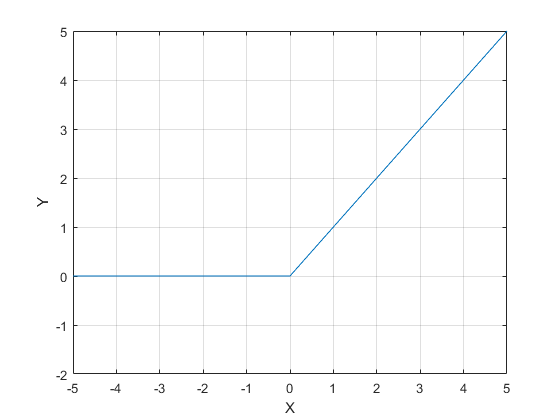
\includegraphics[width=6.5cm]{ReLU}
        \label{Figure:ReLUplots:ReLU}
    }
    \subcaptionbox{Leaky ReLU}{
        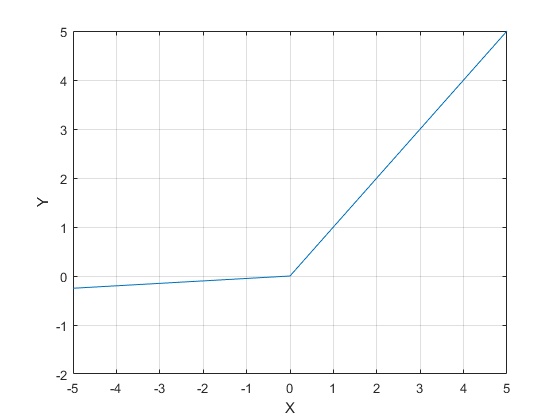
\includegraphics[width=6.5cm]{LeakyReLU}
        \label{Figure:ReLUplots:LeakyReLU}
    }
    \caption{ReLU activation functions}
    \label{Figure:ReLUplots}
\end{figure}

It is also possible to use the exponential linear units (ELU) to address the problem of inactive neurons. 
It uses $e^x-1$, which gives a similar curve, but has a small negative value at $x < 0$. 

\subsubsection{Other Functions}

There are many other activation functions such as sigmoid, hyperbolic tangent (Tanh), Softmax, etc.
Those are suitable for different purposes. For example, sigmoid have a limited output range, suitable to use before output. 
However, the curve gets too smooth at two ends, which causes a low learning efficiency. It is more used in classification problems. 

\subsection{Backpropagation}

Backpropagation\cite{Sieci} is a way to update $\mathbf{w}$ in the correct direction. It is a supervised learning algorithm that adjusts the parameters $\mathbf{w}$
by propagating the error backward from the output layer to the input layer. 

It first calculates the error $\vec{\delta} = \mathbf{y} - \hat{\mathbf{y}} $, which represents the difference between output values and target values. 
Then, the error of each neuron in the network is calculated. In the previous example \fref{Figure:ANN-structure}, errors for hidden layers are calculated by Equation \ref{eq:bp_error}.  
\begin{gather}
    \vec{\delta_h} = \mathbf{w^{II}} \cdot \vec{\delta}
    \label{eq:bp_error}
\end{gather}
When the error for each neuron is computed, weights could be updated:
\begin{gather}
    \mathbf{w^{I}_{new}} = \mathbf{w^{I}_{old}} + \eta \vec{\delta_h} \frac{\mathrm{d} A_k(\mathbf{w^I_{old}x} + b^I_k)}{\mathrm{d} (\mathbf{w^I_{old}x} + b^I_k)} \mathbf{x} \notag\\
    \mathbf{w^{II}_{new}} = \mathbf{w^{II}_{old}} + \eta \vec{\delta} \mathbf{h} 
\end{gather}
where $\frac{\mathrm{d} A_k(\mathbf{w^I_{old}x} + b^I_k)}{\mathrm{d} (\mathbf{w^I_{old}x} + b^I_k)}$ is the derivative of the activation function.
The learning rate $\eta$ affects the learning speed. The initial values of $\mathbf{w^{I}}$ and $\mathbf{w^{II}}$ could be set randomly. 

The random initial values of $\mathbf{w}$ bring randomness to the training process, making the results of each training different. 
This may help to overcome the local minimum, since every time the route of updates is different, there is a chance that the model will reach lower points next time. 

\section{Network Architectures / Layers}

Targeting different problems, various structures of networks have been designed \cite{Bishop}, i.e. network architectures. 
Different network architectures are designed to solve specific types of tasks or to address particular challenges.
A network architecture contains one or several different layers. Each layer focuses on extracting patterns of a certain aspect of the data. 

\fref{Figure:ANN-structure} shows a structure of a simple Feedforward Neural Networks (FNNs), with a fully connected layer connecting every node to every node. 
By choosing the connections between nodes, ways to update parameters, and the activation functions, different types of layers are formed.  
Different layers may have their own specialisation. 
For example, connecting the nodes convolutionally (CNN layer) would make it particularly well-suited for grid-like data, such as images \cite{726791}. Including a CNN layer in the network is beneficial for extracting spatial patterns of the data.

By combining different layers, e.g. CNN and RNN layers, each layer responsible for extracting certain types of patterns and features, the network would be able to have a good accuracy on complex problems such as traffic prediction.
The following sections will discuss more about different designs of network architectures and layers.

\subsection{Convolutional Neural Networks (CNNs)}

CNNs are widely used in tasks related to image recognition and classification. In traffic prediction, its idea could be used to extract the geographical characteristics of roads. 
Compared to fully connected networks, CNNs have significantly fewer nodes and connections, hence rapidly reducing the computational power required. 
An example of a CNN network's overall structure is shown in \fref{Figure:CNN-structure}.

\begin{figure}[!htb]
    \centering
    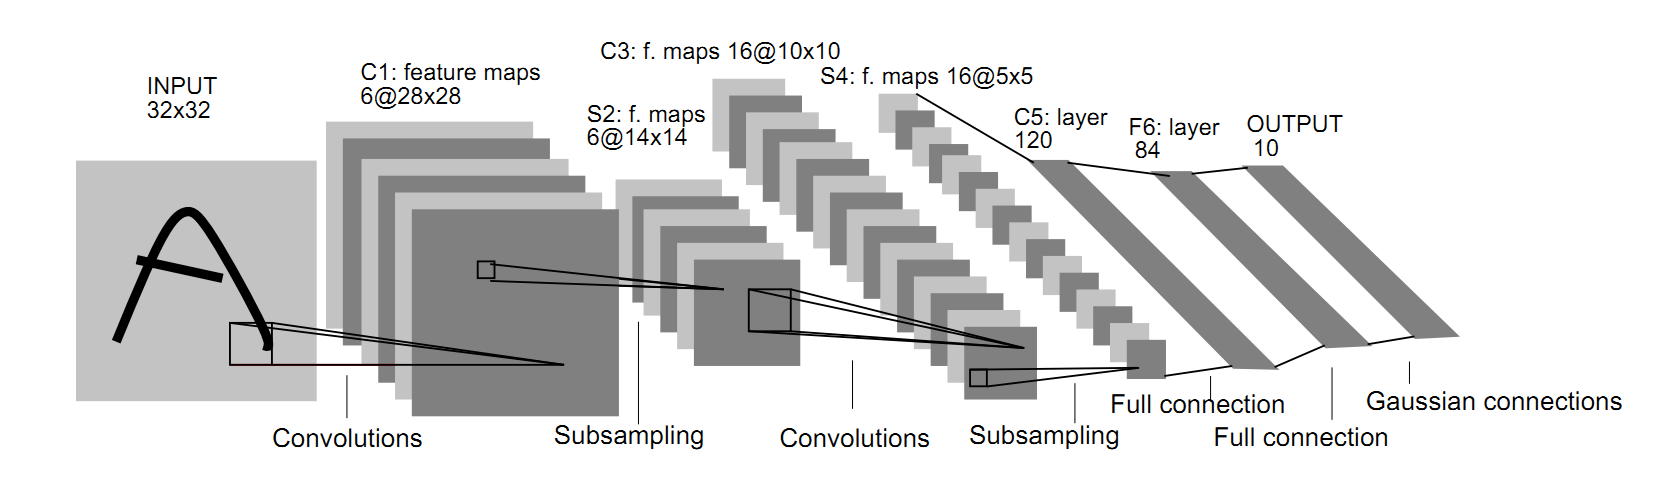
\includegraphics[width=14.5cm]{CNN-structure}
    \caption{Architecture of LeNet-5, a convolutional NN, here used for digits recognition. Each plane is a feature map, i.e., a set of units whose weights are constrained to be identical. (Adapted from \cite{726791})}
    \label{Figure:CNN-structure}
\end{figure}

The core of CNNs is the convolutional layers. They consist of a set of learnable kernels as parameters to train. Each kernel is small spatially but has the same depth as the input vectors. 
Kernels are convolved with the input data to produce feature maps. Let the size of the filter $\mathbf{w}$ being $(m_f \times n_f \times \dots)$, the $(a \times b)$th node in the output feature map $\mathbf{h}$ could be calculate by:
\begin{gather}
    \mathbf{H}_{ab} = A(\sum_{i=a}^{m_f+a} \sum_{j=b}^{n_f+b} (\mathbf{X}_{ij} \odot \mathbf{W}_{ij}))
\end{gather}
The activation function $A$ is also needed to bring non-linearity. 

Repeat this process step by step from the top left corner to the bottom right, spatial information is extracted. 
If some area of input vectors have values similar to the kernel, the corresponding value on the feature map will be large.
Implies that the feature interest has been detected. To update the kernel, backpropagation is used. 

As the input vectors convolute, the result will be smaller, especially when there are multiple convolution layers. The size of the vector can be maintained appropriately through padding. 
Padding refers to the process of adding additional values around the boundary of the input vectors, normally with zeros, before convolution. 

\begin{figure}[!htb]
    \centering
    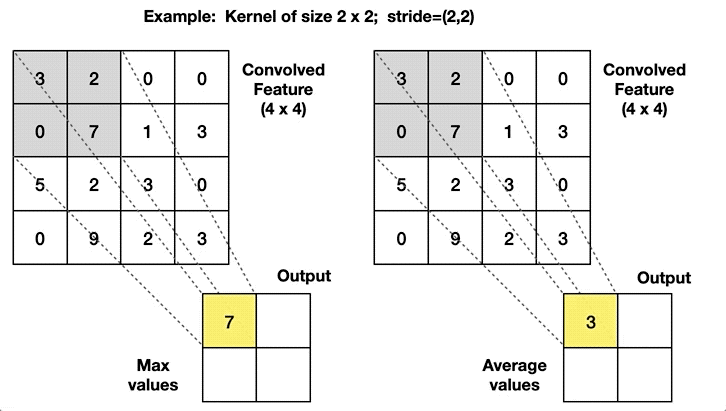
\includegraphics[width=12cm]{pooling}
    \caption{Illustration of Max Pooling: Take the highest value from the area; Average Pooling: Calculate the average value from the area. (Adapted from \cite{poolingplot})}
    \label{Figure:pooling}
\end{figure}

The use of pooling layers is common after convolution to reduce the spatial dimensions. It is like converting a high-resolution image into a lower-resolution one. 
The retained image will not have much impact on the understanding of the content. This can be done by averaging neighbourhoods or selecting the maximum value among neighbourhoods. 

\subsection{Recurrent Neural Networks (RNNs)}

RNNs are a type of architecture that is designed for sequenced data where the order of the data points is crucial \cite{lipton2015critical}. 
This makes RNN a good approach for traffic prediction. 
Similar to fully connected neural networks, RNNs are constructed by multiple RNN nodes in one or more RNN layers. The equation of a RNN layer is given by:
\begin{gather}
    \mathbf{h}_t = A(\mathbf{w^Ix}_t + \mathbf{w^{II}h}_{t-1} + b) \label{eq:RNN}
\end{gather}
where $\mathbf{x}_t$ is the input vector at time $t$, $\mathbf{h}_t$ is the output vector at $t$, hence, $\mathbf{h}_{t-1}$ is the output at time $t-1$. 
Comparing this to Equation \ref{eq:single-layer}, the difference is that the RNN layer includes a term containing information from previous samples in the sequence, $\mathbf{w^{II}h}_{t-1}$.
The essence of RNN is that the output of the current moment will take place in the calculation of the next moment as one of the inputs. 
\fref{Figure:RNN-structure} illustrates the idea of RNN.

\begin{figure}[!htb]
    \centering
    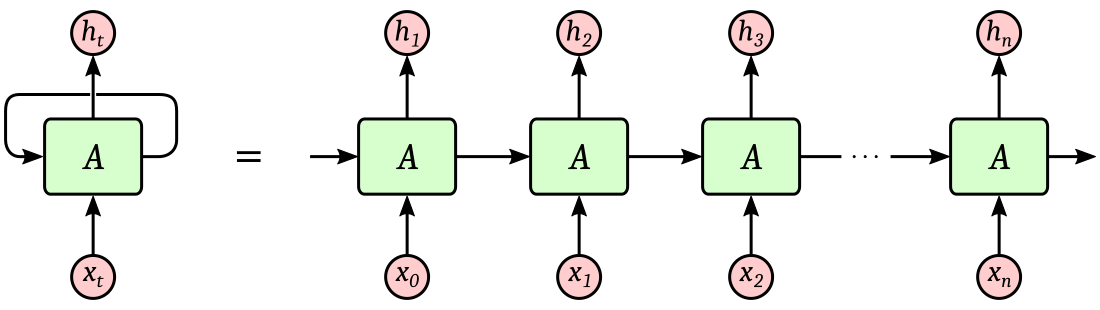
\includegraphics[width=12cm]{rnn}
    \caption{RNN as a neural network very deep in time (Adapted from \cite{rnnplot})}
    \label{Figure:RNN-structure}
\end{figure}

RNNs are susceptible to the vanishing/exploding gradient problem \cite{ribeiro2020exploding}. 
Since the RNN uses the backpropagation to minimise the cost function, and the error has been calculated from outputs going back through the network to update the weights, 
those weights in the feedback loop ($\mathbf{w_{rec}}$) are multiplied a lot of times during the backpropagation. 
If $\mathbf{w_{rec}} < 1$, the gradient will be vanishing, since it approaches 0. In contrast, If $\mathbf{w_{rec}} > 1$, then the weight will tend to be very large, i.e. exploding. 

\subsubsection{Long Short-Term Memory (LSTM)}

\begin{figure}[!htb]
    \centering
    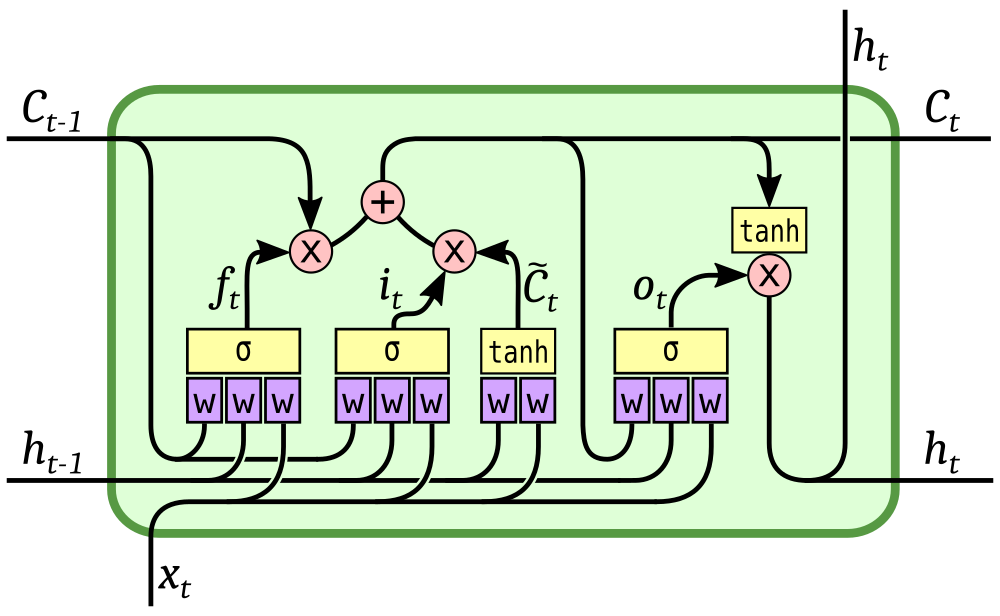
\includegraphics[width=12cm]{lstm}
    \caption{LSTM with peephole connections (Adapted from \cite{rnnplot})}
    \label{Figure:LSTM-structure}
\end{figure}

To address the vanishing/exploding gradient problem, multiple variations of RNN have been proposed. 
Long Short-Term Memory (LSTM) networks are one of the popular architectures \cite{lstm}. 
The structure of LSTM is shown in \fref{Figure:LSTM-structure}. 

The LSTM network introduces three gates to manage the weights of samples in the sequenced data. $f$ is the forget gate, $i$ is input gate, and $o$ is forget gate. 
$\sigma$ represents a sigmoid function that gives a value between 0 and 1, which can act like a switch. 
$\mathbf{h}$ and $\mathbf{c}$ stands for hidden state and cell state. Each carries a memory path to pass down information.  
The equations of the model are given by: 
\begin{gather}
    i_t = \sigma (\mathbf{w}_{xi} \mathbf{x}_t + \mathbf{w}_{hi} \mathbf{h}_{t-1} + \mathbf{w}_{ci} \mathbf{c}_{t-1} + b_i) \notag\\
    f_t = \sigma (\mathbf{w}_{xf} \mathbf{x}_t + \mathbf{w}_{hf} \mathbf{h}_{t-1} + \mathbf{w}_{cf} \mathbf{c}_{t-1} + b_f) \notag\\
    \mathbf{\tilde{c}}_t = \tanh (\mathbf{w}_{xc} \mathbf{x}_t + \mathbf{w}_{hc} \mathbf{h}_{t-1} + b_c) \\
    \mathbf{c}_t = f_t \odot \mathbf{c}_{t-1} + i_t \odot \mathbf{\tilde{c}}_t \notag\\
    o_t = \sigma (\mathbf{w}_{xo} \mathbf{x}_t + \mathbf{w}_{ho} \mathbf{h}_{t-1} + \mathbf{w}_{co} \mathbf{c}_t + b_o) \notag\\
    \mathbf{h}_t = o_t \odot \tanh (\mathbf{c}_t) \notag
\end{gather}
These gates, or rather sigmoid functions, let LSTM choose to ignore a sample if the current sample has been considered as not important. 
Otherwise, the LSTM will discard the information before the sample, and only retain the information of current time $t$. 

In the first version of LSTM, there is no output gate \cite{ribeiro2020exploding}, and the equations are listed below: 
\begin{gather}
    i_t = \sigma (\mathbf{w}_{xi} \mathbf{x}_t + \mathbf{w}_{hi} \mathbf{h}_{t-1} + b_i) \notag\\
    f_t = \sigma (\mathbf{w}_{xf} \mathbf{x}_t + \mathbf{w}_{hf} \mathbf{h}_{t-1} + b_f) \notag\\
    \mathbf{\tilde{h}}_t = \tanh (\mathbf{w}_{xc} \mathbf{x}_t + \mathbf{w}_{hc} \mathbf{h}_{t-1} + b_c) \\
    \mathbf{h}_t = f_t \odot \mathbf{h}_{t-1} + i_t \odot \mathbf{\tilde{h}}_t \notag
\end{gather}
It is clearer that in this set of equations, $\mathbf{i}$ controls the weight of short-term memories, and $f$ controls longer memories. 
Those two gates are independent. While training, it can find suitable parameters for $\mathbf{i}$ and $f$, 
which means $\mathbf{i}$ and $f$  will use different $\mathbf{x} _t$ and $\mathbf{h} _{t-1}$ to give different control strategies.

The addition of the output gate and use of $\mathbf{c}$ is to keep the longer memories more effectively. 
$\mathbf{c}$ does not exit the output gate, hence it is not affected if the current output gate is approaching 0. 
Even though the current $f$ is tend to 0, which means $\mathbf{c}_{t-1}$ has been forgotten, $\mathbf{h} _{t-1}$ still contains information about $\mathbf{c}_{t-1}$. 
This allows the long-term memories to pass down through the time sequence. 

\subsection{Graph Neural Networks (GNNs)}

GNNs are the type of architecture that is designed to work with data that can be represented as graphs, where a graph consists of vertices and edges that connect vertices. 
Each vertex in the graph could be a vector of features. 
In the context of traffic prediction, road networks could easily convert into graphs, with sensors on the road being the vertices and roads between sensors being the edges. 
Suppose exists spatio-temporal series data $\mathbf{X} = \left \{ \mathbf{X}_t \in \mathbb{R}^{N\times F} | t = 0, \dots, T\right \}$, where $N$ is the number of vertices, $F$ is the dimension of the features. 
The graph at time $t$ could be represent as $G_t = (\mathbf{V}, \mathbf{E}_t, \mathbf{A}_t)$. $\mathbf{V}$ contains all vertices, $\mathbf{E}_t$ and $\mathbf{A}_t$ are the edge set and adjacency matrix at time $t$. 
$\mathbf{E}_t$ and $\mathbf{A}_t$ may not vary with time, in that case, the graph $G = (\mathbf{V}, \mathbf{E}, \mathbf{A})$. 

If the topology of the graph is given, e.g. the road network information is given, the adjacency matrix could construct based on the topology by: 
\begin{gather}
    a_{ij}^t = \left\{\begin{aligned}
    1, &\quad \mathrm{if\ \mathbf{V}_i\ connects\ to\ \mathbf{V}_j}\\ \label{eq:top_adj}
    0, &\quad \mathrm{otherwise}
    \end{aligned}\right.
\end{gather}
where $a_{ij}^t$ is the element in the adjacency matrix $\mathbf{A}$ at time $t$. If the topology is not given, it is possible to construct $\mathbf{A}$ by calculating the distance between vertices.
\begin{gather}
    a_{ij}^t = \left\{\begin{aligned}
    \frac{\exp(-\left \| d_{ij}^t \right \|_2 )}{\delta}, &\quad \mathrm{if}\ d_{ij}^t \le \epsilon \\
    0, &\quad \mathrm{otherwise}
    \end{aligned}\right.
\end{gather}
where $d_{ij}^t$ is the distance between vertices $i$ and $j$ at time $t$, $\epsilon$ is a threshold that controls the sparsity of $\mathbf{A}$, and $\delta$ is a parameter that controls the distribution. 

In the traffic prediction problem, an architecture capturing both spatial and temporal characteristics is desired. 
To do this, one could merge spatial graph convolutional network (GCN) used to capture spatial info, with RNN methods to capture temporal characteristics.

\subsubsection{Spatial Graph Convolutional Networks (Spatial GCNs)}

The input of the GCN network is the adjacency matrix $\mathbf{A}$ and the features of each vertex $\mathbf{X}$. 
Intuitively, it is possible to construct the GCN layer by calculating the dot product of $\mathbf{A}$ and $\mathbf{X}$, then dot with the weights $\mathbf{W}$. 
Thus the equation of a GCN layer could be:
\begin{gather}
    \mathbf{H} = A(\mathbf{AXW})
\end{gather}
However, there are some limitations to using this equation \cite{Thomas}. 
Due to the vertices of the graph not connecting to themselves, the diagonal of $\mathbf{A}$ is all zeros. Hence when it multiplies with $\mathbf{X}$, the features of the vertex itself will be ignored. 
It is easy to solve by adding an identity matrix $\mathbf{I}$ to $\mathbf{A}$, so that the diagonal becomes all ones. 
Furthermore, $\mathbf{A}$ has not been normalised. This will change the original scale and distribution of the feature vectors after multiplication. The idea of normalisation is explained in \sref{Section:Normalisation}. 
The normalisation of $\mathbf{A}$ can be done by $\mathbf{D}^{-\frac{1}{2}}\mathbf{AD}^{-\frac{1}{2}}$. Combining these two changes, the equation is now been \cite{Kipf2016SemiSupervisedCW}:
\begin{gather} 
    \mathbf{H} = A\left[\mathbf{D}^{-\frac{1}{2}}(\mathbf{A} + \mathbf{I})\mathbf{D}^{-\frac{1}{2}}\mathbf{XW}\right] \label{eq:gcn}
\end{gather}

\begin{figure}[!htb]
    \centering
    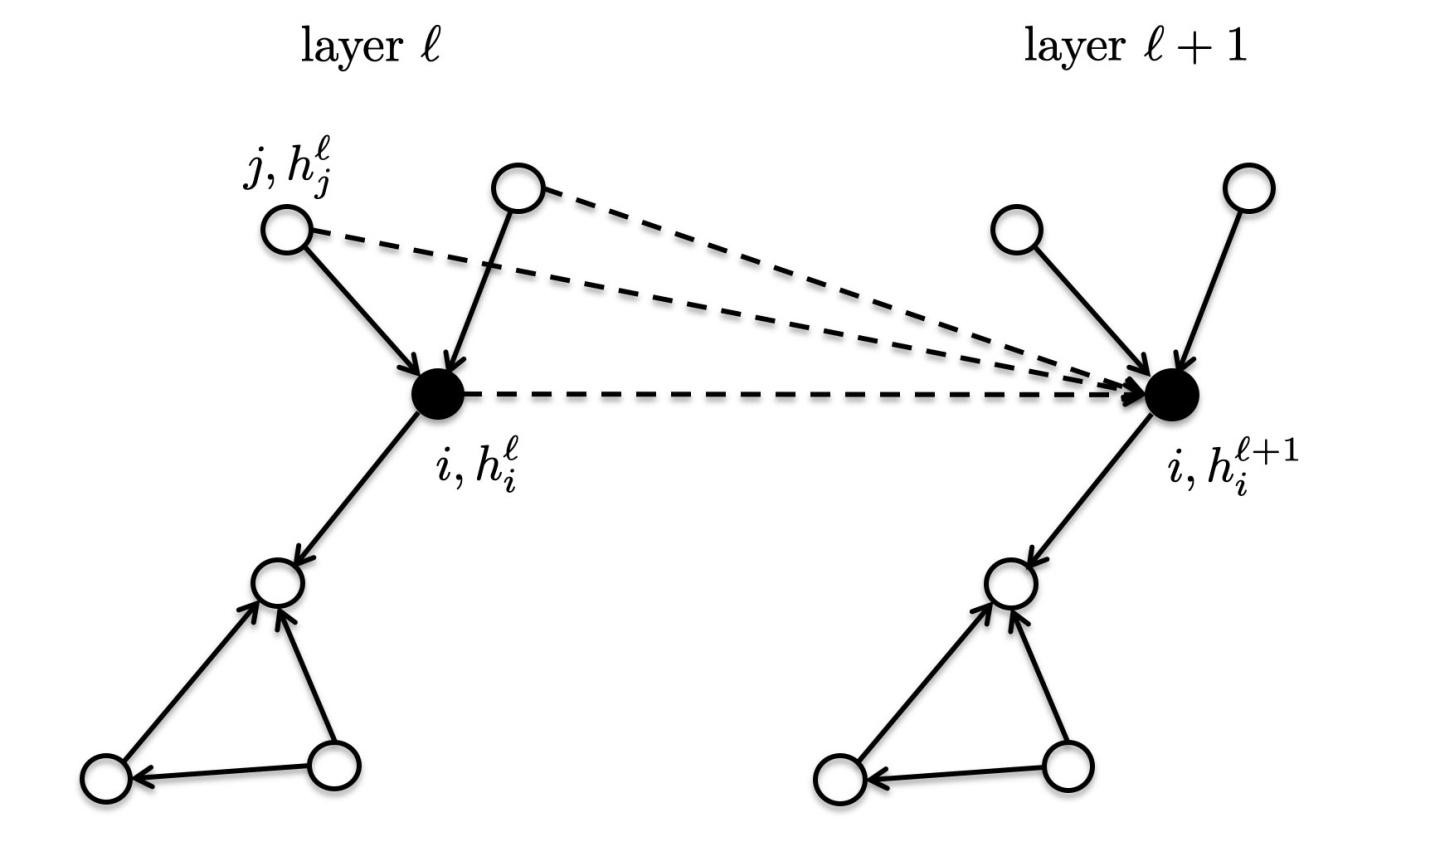
\includegraphics[width=12cm]{gcn.jpg}
    \caption{Illustration of the connections of vertex $i$ in a GCN layer.}
    \label{Figure:gcn-structure}
\end{figure}

Refer to \fref{Figure:gcn-structure}, all the vertices that connect to the vertex $i$ are considered to calculate the output of $\mathbf{h}_i^{l+1}$
The graph in this example is a directional graph, where the connections only hold in one direction. The GCN layer only considers the vertices that connect to $i$ and $i$ itself, but not the ones that $i$ connects to.

\section{Data Process}

\subsection{One-hot Encoding}

Sometimes the data used contains categorical variables, which represent categories or labels, such as weekdays, and the class of a road.
Each value of these variables is independent, the size does not matter. To let the model understand this better, one-hot encoding could be introduced.

One-hot encoding is a technique used to represent those categorical variables as binary vectors. The length of the vectors is equal to the number of unique categories,
and each position in the vector corresponds to a specific category. If the data is in a category, the corresponding position is set to be 1, otherwise, fill with 0. 
With this implemented, each category is treated as an independent entity and does not impose any ordinal relationship. 

\subsection{Normalisation} \label{Section:Normalisation}

Different features in the dataset often have different units and scales. This makes in some of the dimensions, the data more concentrated than others. 
In the process of gradient descent, it is hence more likely to deviate from the minimum and result in longer training time.

To minimise the effect of them, normalise data before training could be done. 
Normalisation is the process of limiting the preprocessed data to a certain range (such as $[0, 1]$ or $[-1, 1]$).
There are many ways to normalise data. In this project, Min-Max Normalisation is used. 
\begin{gather}
    \mathbf{x}' = \frac{\mathbf{x}-\mathrm{min}(\mathbf{x})}{\mathrm{max}(\mathbf{x})-\mathrm{min}(\mathbf{x})}
\end{gather}
Min-Max Normalisation converts the data into $[0, 1]$ range, the minimum value being 0, and the maximum being 1.

Due to the values after normalisation depending on the min and max values in the dataset, normalise the whole dataset will leak some subsequent information of the data to the previous samples. 
Consequently, normalisation of the validation set and the test set will use the factor generated by the training set, as presented in Equation \ref{Equation:norm_test}.
\begin{gather}
    \mathbf{x_{validation}}' = \frac{\mathbf{x_{validation}}-\mathrm{min}(\mathbf{x_{train}})}{\mathrm{max}(\mathbf{x_{train}})-\mathrm{min}(\mathbf{x_{train}})}, \quad
    \mathbf{x_{test}}' = \frac{\mathbf{x_{test}}-\mathrm{min}(\mathbf{x_{train}})}{\mathrm{max}(\mathbf{x_{train}})-\mathrm{min}(\mathbf{x_{train}})}
    \label{Equation:norm_test}
\end{gather}
In this way, the training set does not contain any information about the test and validation set, and the three sets still remain consistent.
